\documentclass[conference]{IEEEtran}

\usepackage[T1]{fontenc}
\usepackage[utf8]{inputenc}
\usepackage{amsmath}
\usepackage{amssymb}
\usepackage{graphicx}
\usepackage{tikz}
\usepackage{booktabs}
\usepackage{cite}
\usepackage{url}
\usepackage{hyperref}
\usetikzlibrary{arrows.meta, positioning, calc}
\title{Implementing and Evaluating Skeen's Atomic Multicast Protocol and an ACK-Gated Extension for Atomic Global Order}
\author{Agatha Schneider\\
Pontifícia Universidade Católica do Rio Grande do Sul (PUCRS)\\
Porto Alegre, Brazil\\
htaschneider@icloud.com
}
\date{}

\begin{document}

\maketitle

\begin{abstract}
Atomic multicast is a central communication abstraction for partitioned state machine replication and distributed key-value stores because it orders operations only at the partitions they access while preserving consistency across overlapping destination sets. Skeen's decentralized atomic multicast protocol provides a compact timestamp-based ordering mechanism, but later work shows that the original protocol admits unsafe executions when overlapping multicasts expose real-time dependencies before all destinations have converged on the same delivery barrier. This paper implements and evaluates two protocols in a distributed key-value store: original Skeen and the ACK-gated extension proposed by Pacheco et al. The system supports generic N-partition routing, configurable membership, arbitrary multicast destination sets, in-memory and HTTP transports, Docker deployment, and structured logging. Its main engineering contribution is a deterministic validation framework that controls message delivery using scheduled transport queues, predicate-based release rules, delivery trace recording, and cycle detection. The framework reproduces a representative unsafe execution for original Skeen without sleeps or timing races and shows that the ACK-gated variant prevents premature delivery for that same scheduled counterexample. This is counterexample reproduction and regression validation, not exhaustive safety verification. We also benchmark both protocols for cluster sizes 2, 3, and 5 and destination sets up to the full cluster under injected delays of 0, 1, 5, and 10 ms. The results quantify the cost of the acknowledgement barrier: ACK gating adds measurable CPU and allocation overhead in the zero-delay case, and the extra control-message dependency becomes visible under artificial phase-counting latency.
\end{abstract}

\section{Introduction}

Distributed key-value stores and partitioned state machine replication systems must often coordinate operations that access only a subset of partitions. A single-key update may involve one partition, whereas a range query or multi-key transaction may span several partitions. Broadcasting every operation to every server is simple but wasteful; routing each operation only to its destination set avoids unnecessary processing at unrelated partitions but requires a multicast layer that preserves a consistent order whenever destination sets overlap.

Atomic multicast addresses this requirement by ensuring that processes delivering the same messages deliver them in the same order. Skeen's protocol is a classic decentralized solution based on logical timestamps, local timestamp proposals, a final timestamp decision, and delivery queues ordered by final sequence numbers \cite{lamport,skeen}. Its appeal is that it avoids a single sequencer and lets each multicast destination participate in timestamp selection.

However, Pacheco et al. show that global total order alone is not sufficient for partitioned state machine replication when real-time dependencies cross overlapping groups \cite{pacheco}. In particular, the original protocol can deliver a message at one destination, accept a later overlapping multicast, and then allow another destination to observe the later message before the earlier one. The resulting execution may be compatible with each local delivery queue but incompatible with the stronger atomic global order needed to avoid application-level coordination.

This paper evaluates that issue through an independent implementation rather than a proof sketch alone. We implement original Skeen and the ACK-gated variant in a distributed key-value store, reproduce a known unsafe execution using a deterministic scheduler, and measure the cost of adding the acknowledgement barrier. The validation result is intentionally scoped: it demonstrates that the counterexample can occur in executable code and that the implemented ACK gate blocks the same schedule, but it does not replace the formal safety argument in prior work or exhaustively explore all possible interleavings.

The contributions are:
\begin{itemize}
    \item A configurable distributed key-value store with generic partition routing, static membership configuration, arbitrary multicast destination sets, and selectable original or ACK-gated Skeen modes.
    \item A dual transport stack with an in-memory transport for tests and controlled simulation, an HTTP transport for deployment, Docker configuration, and logging abstractions.
    \item A deterministic validation framework that reproduces a representative unsafe original-Skeen execution using scheduled message delivery, predicate-based release, delivery recording, and cycle detection.
    \item A benchmark pipeline that collects Go benchmark output, parses it into CSV matrices, and generates Matplotlib plots for per-operation latency, memory consumption, allocation rate, and latency sensitivity.
\end{itemize}

The evaluation is organized around three research questions. \textbf{RQ1}: Can the unsafe execution described for original Skeen be reproduced as a deterministic counterexample in an independent implementation? \textbf{RQ2}: Does the ACK-gated extension block that same scheduled counterexample under an identical deterministic message schedule? \textbf{RQ3}: What CPU, memory, allocation, and latency overheads does the acknowledgement barrier introduce in the measured configurations?

\section{Background and Related Work}

Atomic multicast provides reliable, consistently ordered delivery to a subset of processes \cite{hadzilacos}. If two multicast messages are delivered at two common destinations, those destinations must deliver them in the same relative order. This property is especially useful in partitioned storage systems: each operation is multicast only to the partitions whose state it may read or write, but overlapping operations still observe a common serialization order.

Skeen's protocol assigns total order without a centralized sequencer \cite{skeen}. A client or coordinator sends a \textsc{Start} message to every destination in the multicast set. Each destination increments a logical clock, stores the request in a delivery queue as undeliverable, and returns a proposed timestamp. After proposals have been collected, the maximum proposal becomes the final timestamp and is multicast to all destinations. A process may then deliver the message when it is stable at the head of its queue. Ties are broken by process identifiers, producing a deterministic ordering relation over timestamp pairs.

The vulnerability identified by Pacheco et al. is not simply a disagreement about the final timestamp of one message \cite{pacheco}. The problem appears when real-time dependencies interact with overlapping destination sets. Suppose message $m$ is delivered at one destination before a later message $m'$ is multicast, but another destination learns enough timestamps to deliver $m'$ before $m$. The local delivery rules can remain internally consistent while the global execution graph contains a cycle: a real-time edge $m \rightarrow m'$ and a delivery-order edge $m' \rightarrow m$. This violates the stronger ordering needed by partitioned state machine replication to execute delivered operations immediately without additional synchronization.

Pacheco et al. propose an ACK-gated extension that strengthens delivery by adding an explicit acknowledgement barrier after the final timestamp is learned \cite{pacheco}. Once a destination learns the final timestamp, it broadcasts an \textsc{ACK} to the other destinations. A message is deliverable only after the process has received acknowledgements from every destination in the multicast set. This barrier prevents a destination from delivering a finalized message while another destination in the same multicast can still assign or expose a lower ordering constraint for an overlapping execution.

\section{System Architecture and Implementation}

\subsection{Distributed Key-Value Store}

The key-value store exposes a partitioned storage interface over the multicast abstraction. Requests carry an operation type, request identifier, and explicit destination set. \textsc{Put} operations target exactly one partition, while range operations may target arbitrary destination sets. The routing layer supports configurable $N$-partition clusters, so the same protocol code can be evaluated for $N=2$, $N=3$, and $N=5$ without hard-coded participant assumptions.












Each partition owns a Skeen protocol instance, a local key-value store, a logical clock, and a map of request states. A request state records the request payload, the local timestamp proposal, all collected proposals, the final timestamp, ACK state, delivery status, result data, and a completion channel used by synchronous client submission. Protocol mode is selected at construction time: original mode ignores ACK state during delivery, while ACK-gated mode requires every destination ACK before delivery.

\subsection{Protocol Execution}

Protocol execution uses four message types: \textsc{Start}, \textsc{Local\_TS}, \textsc{Final\_TS}, and \textsc{ACK}. On \textsc{Start}, a destination validates membership in the destination set, advances its clock, stores a local proposal, and broadcasts that proposal. When proposals from all destinations are present, the maximum timestamp is learned as the final timestamp and broadcast. A final timestamp also advances local clock state if necessary.












Delivery is attempted after every protocol message. The node collects finalized, undelivered requests and sorts them by final timestamp. A candidate can be delivered only if it is finalized, not already delivered, and lower than every other pending local or final timestamp known at the node. In ACK-gated mode, the candidate must also have ACKs from all destinations. Delivery executes the key-value operation, records any range result, invokes the delivery hook used by tests, and releases the waiting submitter.

\subsection{Dual Transport Stack and Deployment}

The transport interface contains a single protocol send operation. The in-memory transport maps partition identifiers directly to local Skeen instances and is used for unit tests, benchmarks, and deterministic simulation. The HTTP transport serializes protocol messages as JSON and sends them to each peer partition's internal protocol endpoint. This separation lets the protocol be tested without network non-determinism while preserving a deployable HTTP path. The repository also includes Docker Compose configurations for multi-process execution and logging helpers that can be disabled during benchmarks.

Both transports invoke the same protocol state machine. In the in-memory case, a send to partition identifier $p$ performs a map lookup and calls the receiver's protocol handler directly. In the HTTP case, the same \textsc{Start}, \textsc{Local\_TS}, \textsc{Final\_TS}, and \textsc{ACK} records are JSON encoded and delivered to the peer endpoint configured for partition $p$, where the receiver invokes the same handler. The transport changes serialization and process placement, but not timestamp selection, request-state transitions, ACK bookkeeping, or delivery predicates. This equivalence allows deterministic and zero-delay experiments to use the in-memory transport while preserving a deployable HTTP path.

\subsection{Deterministic Validation Framework}

Figure~\ref{fig:counterexample} summarizes the counterexample reproduced by the deterministic scheduler and the corresponding ACK-gated behavior. The first panel shows how original Skeen can expose a real-time dependency while another destination observes the opposite delivery order. The second panel shows how the ACK barrier delays delivery until all destinations have acknowledged the final timestamp.

\begin{figure}[!b]
\centering
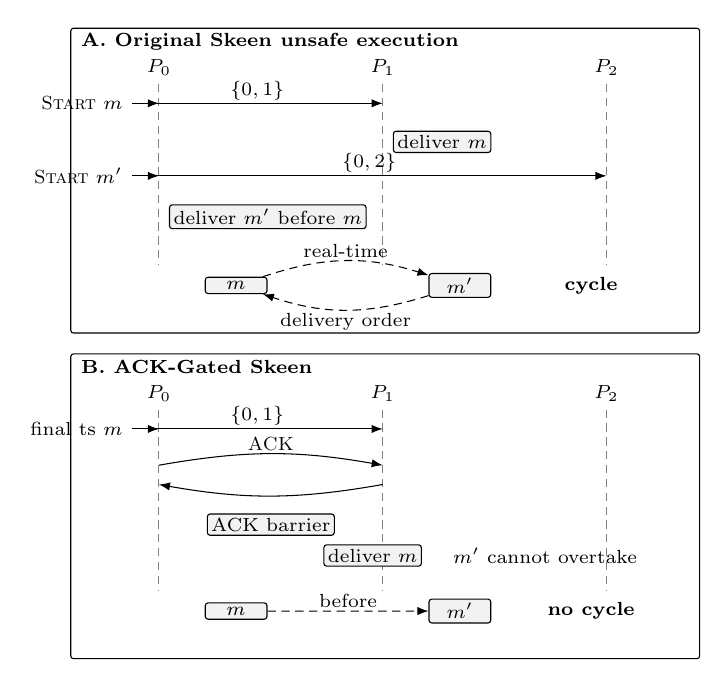
\begin{tikzpicture}[
    font=\scriptsize,
    scale=0.98,
    transform shape,
    >=Latex,
    x=1cm,
    y=1cm,
    panel/.style={draw, rounded corners=1pt, inner sep=3pt},
    lifeline/.style={gray, densely dashed, line width=0.35pt},
    msg/.style={-{Latex[length=1.4mm]}, line width=0.38pt},
    dep/.style={-{Latex[length=1.4mm]}, densely dashed, line width=0.38pt},
    event/.style={draw, fill=gray!10, rounded corners=1pt, inner sep=1.5pt},
    label/.style={inner sep=1pt, align=center}
]

\node[panel, minimum width=8.15cm, minimum height=3.95cm, anchor=north west] (orig) at (0,0) {};
\node[label, font=\scriptsize\bfseries, anchor=west] at ($(orig.north west)+(0.10,-0.18)$) {A. Original Skeen unsafe execution};
\foreach \x/\p in {1.15/$P_0$,4.05/$P_1$,6.95/$P_2$} {
    \node[label] at ($(orig.north west)+(\x,-0.52)$) {\p};
    \draw[lifeline] ($(orig.north west)+(\x,-0.73)$) -- ($(orig.north west)+(\x,-3.08)$);
}
\node[label, anchor=east] at ($(orig.north west)+(0.72,-0.98)$) {\textsc{Start} $m$};
\draw[msg] ($(orig.north west)+(0.80,-0.98)$) -- ($(orig.north west)+(1.15,-0.98)$);
\draw[msg] ($(orig.north west)+(0.80,-0.98)$) -- ($(orig.north west)+(4.05,-0.98)$)
    node[midway, above, label] {$\{0,1\}$};
\node[event, anchor=west] (omdel) at ($(orig.north west)+(4.18,-1.48)$) {deliver $m$};
\node[label, anchor=east] at ($(orig.north west)+(0.72,-1.92)$) {\textsc{Start} $m'$};
\draw[msg] ($(orig.north west)+(0.80,-1.92)$) -- ($(orig.north west)+(1.15,-1.92)$);
\draw[msg] ($(orig.north west)+(0.80,-1.92)$) -- ($(orig.north west)+(6.95,-1.92)$)
    node[midway, above, label] {$\{0,2\}$};
\node[event, anchor=west] (ompdel) at ($(orig.north west)+(1.28,-2.45)$) {deliver $m'$ before $m$};
\node[event, minimum width=0.80cm] (om) at ($(orig.north west)+(2.15,-3.34)$) {$m$};
\node[event, minimum width=0.80cm] (omp) at ($(orig.north west)+(5.05,-3.34)$) {$m'$};
\draw[dep, bend left=18] (om) to node[above, label] {real-time} (omp);
\draw[dep, bend left=18] (omp) to node[below, label] {delivery order} (om);
\node[label, font=\scriptsize\bfseries] at ($(orig.north west)+(6.75,-3.34)$) {cycle};

\node[panel, minimum width=8.15cm, minimum height=3.95cm, anchor=north west] (ack) at (0,-4.22) {};
\node[label, font=\scriptsize\bfseries, anchor=west] at ($(ack.north west)+(0.10,-0.18)$) {B. ACK-Gated Skeen};
\foreach \x/\p in {1.15/$P_0$,4.05/$P_1$,6.95/$P_2$} {
    \node[label] at ($(ack.north west)+(\x,-0.52)$) {\p};
    \draw[lifeline] ($(ack.north west)+(\x,-0.73)$) -- ($(ack.north west)+(\x,-3.08)$);
}
\node[label, anchor=east] at ($(ack.north west)+(0.72,-0.98)$) {final ts $m$};
\draw[msg] ($(ack.north west)+(0.80,-0.98)$) -- ($(ack.north west)+(1.15,-0.98)$);
\draw[msg] ($(ack.north west)+(0.80,-0.98)$) -- ($(ack.north west)+(4.05,-0.98)$)
    node[midway, above, label] {$\{0,1\}$};
\draw[msg, bend left=10] ($(ack.north west)+(1.15,-1.45)$) to node[above, label] {\textsc{ACK}} ($(ack.north west)+(4.05,-1.45)$);
\draw[msg, bend left=10] ($(ack.north west)+(4.05,-1.70)$) to ($(ack.north west)+(1.15,-1.70)$);
\node[event] (barrier) at ($(ack.north west)+(2.60,-2.22)$) {ACK barrier};
\node[event, anchor=west] at ($(ack.north west)+(3.28,-2.62)$) {deliver $m$};
\node[label, anchor=west] at ($(ack.north west)+(4.92,-2.62)$) {$m'$ cannot overtake};
\node[event, minimum width=0.80cm] (am) at ($(ack.north west)+(2.15,-3.34)$) {$m$};
\node[event, minimum width=0.80cm] (amp) at ($(ack.north west)+(5.05,-3.34)$) {$m'$};
\draw[dep] (am) -- node[above, label] {before} (amp);
\node[label, font=\scriptsize\bfseries] at ($(ack.north west)+(6.75,-3.34)$) {no cycle};
\end{tikzpicture}
\caption{Conceptual sequence diagram for the reproduced unsafe execution. In original Skeen, a real-time edge $m \rightarrow m'$ can coexist with a delivery-order edge $m' \rightarrow m$ at an overlapping destination, forming a cycle. The ACK-gated variant delays delivery until all destinations acknowledge the final timestamp, preventing the premature delivery used by the counterexample.}
\label{fig:counterexample}
\end{figure}

Distributed protocol tests frequently rely on sleeps, goroutine scheduling, or best-effort network delays. Those techniques make unsafe traces difficult to reproduce and can confuse protocol bugs with timing accidents. The validation framework instead introduces a scheduled transport that records outbound protocol messages rather than delivering them immediately. Tests explicitly release queued messages through predicates over message type, request identifier, sender, receiver, and destination set.

Let a queued message have fields \(to\), \(type\), \(id\), \(from\), and \(dst\), where \(dst\) is the request destination set. A release predicate is a Boolean function over these fields:
\[
\begin{aligned}
P(q) ::= {}& P_{\mathrm{type}}(type) \wedge P_{\mathrm{id}}(id) \\
&\wedge P_{\mathrm{from}}(from) \wedge P_{\mathrm{to}}(to)\\
&\wedge P_{\mathrm{dst}}(dst).
\end{aligned}
\]
Any conjunct may be omitted. The scheduler operation
\[
\mathrm{releaseFirst}(P)
\]
removes the first queued message satisfying $P$ and invokes the receiver's protocol handler; \(\mathrm{drain}\) repeatedly releases the queue head until no messages remain. For example, the predicate used to release a proposal from partition 0 to partition 1 for request $m$ is
\[
q.type=\textsc{Local\_TS} \wedge q.id=m \wedge q.from=0 \wedge q.to=1.
\]
This definition makes the counterexample schedule independent of wall-clock time and operating-system goroutine order.

The framework also records per-partition delivery traces. These traces are converted into a directed graph: if a partition delivers $a$ before $b$, the graph records $a \rightarrow b$. Tests may add real-time edges from the scenario under study, such as $m \rightarrow m'$ when $m'$ is submitted only after $m$ has already been delivered. A depth-first cycle detector then determines whether the combined delivery and real-time constraints violate atomic global order.

The reproduced unsafe schedule uses three partitions. Message $m$ targets partitions 0 and 1; message $m'$ targets partitions 0 and 2. By controlling initial clocks and releasing selected \textsc{Local\_TS} messages, original Skeen allows partition 1 to deliver $m$, then allows partition 0 to deliver $m'$ before $m$. Adding the real-time edge from the delivery of $m$ to the later multicast of $m'$ creates the expected cycle. Running the same schedule in ACK-gated mode leaves partition 1 unable to deliver $m$ until the missing destination ACK is released; after the scheduler drains all messages, no cycle is detected. This experiment is a precise regression trace, not a model checker: it demonstrates the existence of the original bug and the absence of that bug on this trace, while broader schedule-space exploration remains future work.

\section{Experimental Evaluation}

\subsection{Methodology}

The benchmark pipeline begins with Go benchmarks using \texttt{testing.B} and \texttt{ReportAllocs}. Raw benchmark text is converted to CSV by a custom parser that extracts benchmark name, cluster size, protocol mode, destination count, fixed delay, ACK-specific delay, \texttt{ns/op}, \texttt{B/op}, and \texttt{allocs/op}. The plotting stage loads these matrices and generates high-resolution PNG plots with Matplotlib. Each figure is generated directly from parsed CSV output of the corresponding Go benchmark family, with no manual data entry. Go's benchmark harness chooses the inner iteration count for each run; our reported statistics aggregate repeated benchmark runs after normalizing by Go's per-operation counters.

Two benchmark families are used. The first evaluates destination-set overhead for $N \in \{2,3,5\}$ and destination counts from one partition to the full cluster; Table~\ref{tab:inmemory} reports 10 repeated runs. The second fixes $N=3$ and injects artificial latency of 0, 1, 5, and 10 ms into protocol messages; Table~\ref{tab:latency} reports 5 repeated runs. A separate ACK-delay benchmark applies delay only to \textsc{ACK} messages, isolating the cost of the ACK-gated barrier. The current N-sweep stops at 5 because the benchmark campaign was designed to validate the small-cluster correctness scenarios and quantify local protocol overhead, not to claim asymptotic scalability. The growth from $N=3$ to $N=5$ motivates future measurements at $N=7$, $N=10$, and beyond.

\subsection{Correctness Results}

The deterministic validation tests answer the scoped forms of RQ1 and RQ2. For RQ1, original Skeen reproduces the unsafe Pacheco-style trace: one partition delivers $m$, a later overlapping multicast $m'$ is introduced, and another partition delivers $m'$ before $m$. The resulting graph contains a cycle once the real-time edge $m \rightarrow m'$ is included. A control test also verifies that original Skeen does not create a pure delivery-order cycle without the real-time edge, matching the nature of the reported vulnerability.

For RQ2, the ACK-gated implementation prevents the same trace. Under the identical message schedule, a destination that has learned a final timestamp cannot deliver until every destination in the multicast set has acknowledged that final timestamp. This blocks the premature delivery that creates the original cycle. Once the scheduler drains all messages, delivery proceeds consistently and the cycle detector reports no violation. This result should be read as deterministic counterexample reproduction and regression testing rather than exhaustive verification of the ACK-gated protocol.

\subsection{Zero-Delay Overhead}

Table~\ref{tab:inmemory} answers the zero-delay portion of RQ3 by summarizing the in-memory destination-overhead benchmark. With full destination sets, ACK-gated mode increases latency from 0.293 ms to 0.350 ms at $N=2$, from 0.488 ms to 0.608 ms at $N=3$, and from 0.751 ms to 1.193 ms at $N=5$. The cost is also visible in memory and allocation counters because ACK state and ACK messages add per-request bookkeeping. The reported standard deviations are small for the zero-delay benchmark, so the full-destination latency differences are well above run-to-run noise in this dataset.

\begin{table*}[t]
\centering
\caption{In-memory full-destination overhead. Values are mean $\pm$ sample standard deviation over 10 repeated benchmark runs.}
\label{tab:inmemory}
\begin{tabular}{lrrrr}
\toprule
Mode / $N$ & dst & ms/op & B/op & allocs/op \\
\midrule
Original / 2 & 2 & $0.293 \pm 0.001$ & $5039.2 \pm 2.8$ & $53.1 \pm 0.3$ \\
ACK-gated / 2 & 2 & $0.350 \pm 0.001$ & $7214.4 \pm 2.6$ & $71.0 \pm 0.0$ \\
Original / 3 & 3 & $0.488 \pm 0.002$ & $8074.1 \pm 1.6$ & $72.0 \pm 0.0$ \\
ACK-gated / 3 & 3 & $0.608 \pm 0.002$ & $12292.4 \pm 3.2$ & $104.1 \pm 0.3$ \\
Original / 5 & 5 & $0.751 \pm 0.003$ & $16207.6 \pm 4.3$ & $110.0 \pm 0.0$ \\
ACK-gated / 5 & 5 & $1.193 \pm 0.003$ & $26320.0 \pm 4.5$ & $176.0 \pm 0.0$ \\
\bottomrule
\end{tabular}
\end{table*}

Figure~\ref{fig:overhead} shows that the ACK gate has almost no effect for single-destination operations, where the process can acknowledge itself, but the gap grows with destination-set size. This matches the implementation structure: ACK gating only adds meaningful network fan-out when more than one destination participates.

\begin{figure}[t]
\centering
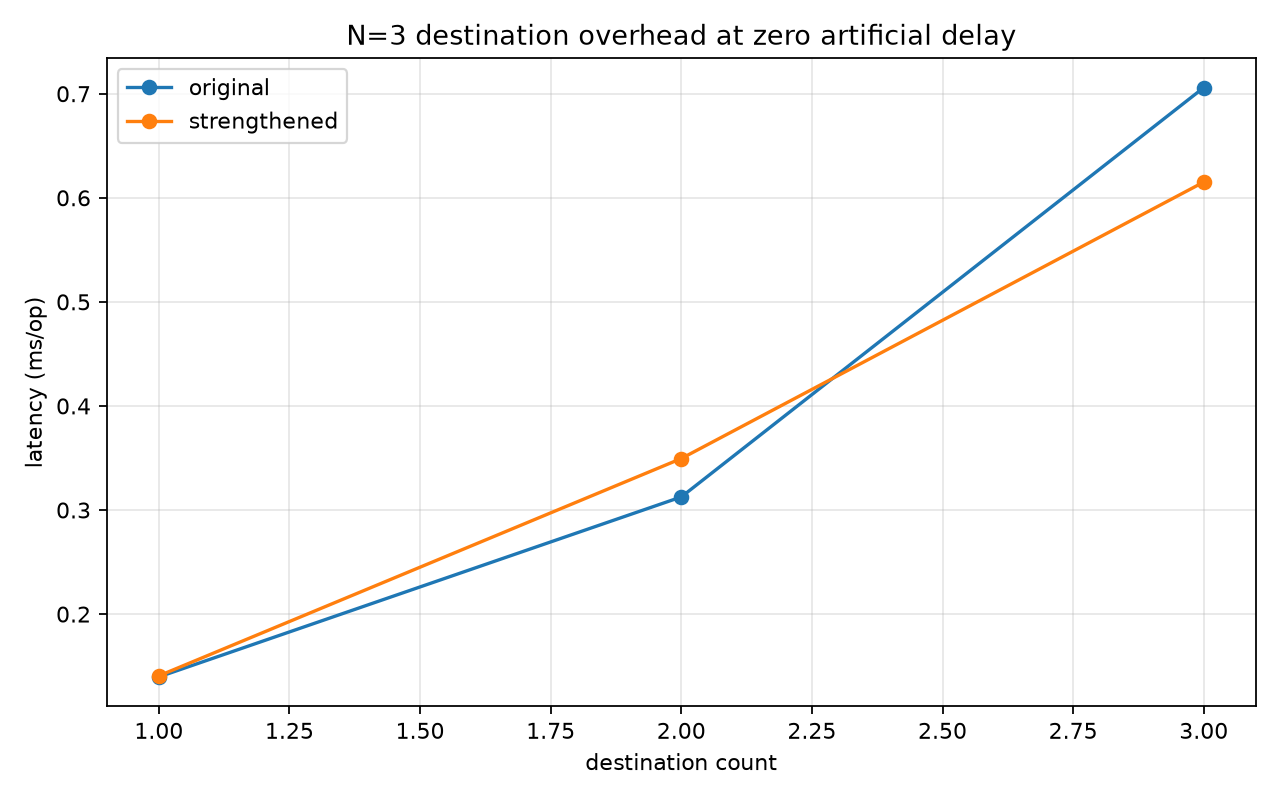
\includegraphics[width=\linewidth,keepaspectratio]{overhead_by_dst.png}
\caption{Destination-set overhead for $N=3$ without artificial latency.}
\label{fig:overhead}
\end{figure}

\subsection{Latency Sensitivity}

Table~\ref{tab:latency} and Fig.~\ref{fig:latency} answer the latency portion of RQ3 for $N=3$, destination count 3, and fixed artificial delay on all protocol messages. The injected delay is a phase-counting tool: it applies a constant delay to each message and intentionally excludes jitter, tail latency, packet loss, and congestion effects. Therefore the results should not be interpreted as a deployed-network performance model. At 5 ms injected delay, original Skeen averages 39.436 ms/op while ACK-gated Skeen averages 61.753 ms/op. At 10 ms, the original protocol averages 76.789 ms/op and the ACK-gated protocol averages 120.357 ms/op. The additional delay is consistent with the extra ACK dependency: ACK-gated Skeen is not only performing more local bookkeeping, it must also wait for another control-message phase before delivery can release the client operation.

\begin{table*}[t]
\centering
\caption{$N=3$, dst=3 latency sensitivity under fixed artificial message delay. Values are mean $\pm$ sample standard deviation over 5 repeated benchmark runs.}
\label{tab:latency}
\begin{tabular}{lrrrr}
\toprule
Mode & delay (ms) & ms/op & B/op & allocs/op \\
\midrule
Original & 0 & $0.706 \pm 0.492$ & $8076.2 \pm 13.8$ & $71.8 \pm 0.4$ \\
ACK-gated & 0 & $0.615 \pm 0.014$ & $12301.6 \pm 27.5$ & $104.2 \pm 0.4$ \\
Original & 1 & $8.085 \pm 0.003$ & $12581.6 \pm 1.5$ & $126.0 \pm 0.0$ \\
ACK-gated & 1 & $12.670 \pm 0.009$ & $18357.2 \pm 4.0$ & $176.0 \pm 0.0$ \\
Original & 5 & $39.436 \pm 0.058$ & $12733.0 \pm 11.7$ & $127.0 \pm 0.0$ \\
ACK-gated & 5 & $61.753 \pm 0.113$ & $18495.8 \pm 11.0$ & $177.8 \pm 0.4$ \\
Original & 10 & $76.789 \pm 0.066$ & $12773.2 \pm 81.4$ & $128.0 \pm 0.0$ \\
ACK-gated & 10 & $120.357 \pm 0.321$ & $18594.2 \pm 24.0$ & $178.8 \pm 0.4$ \\
\bottomrule
\end{tabular}
\end{table*}

\begin{figure}[t]
\centering
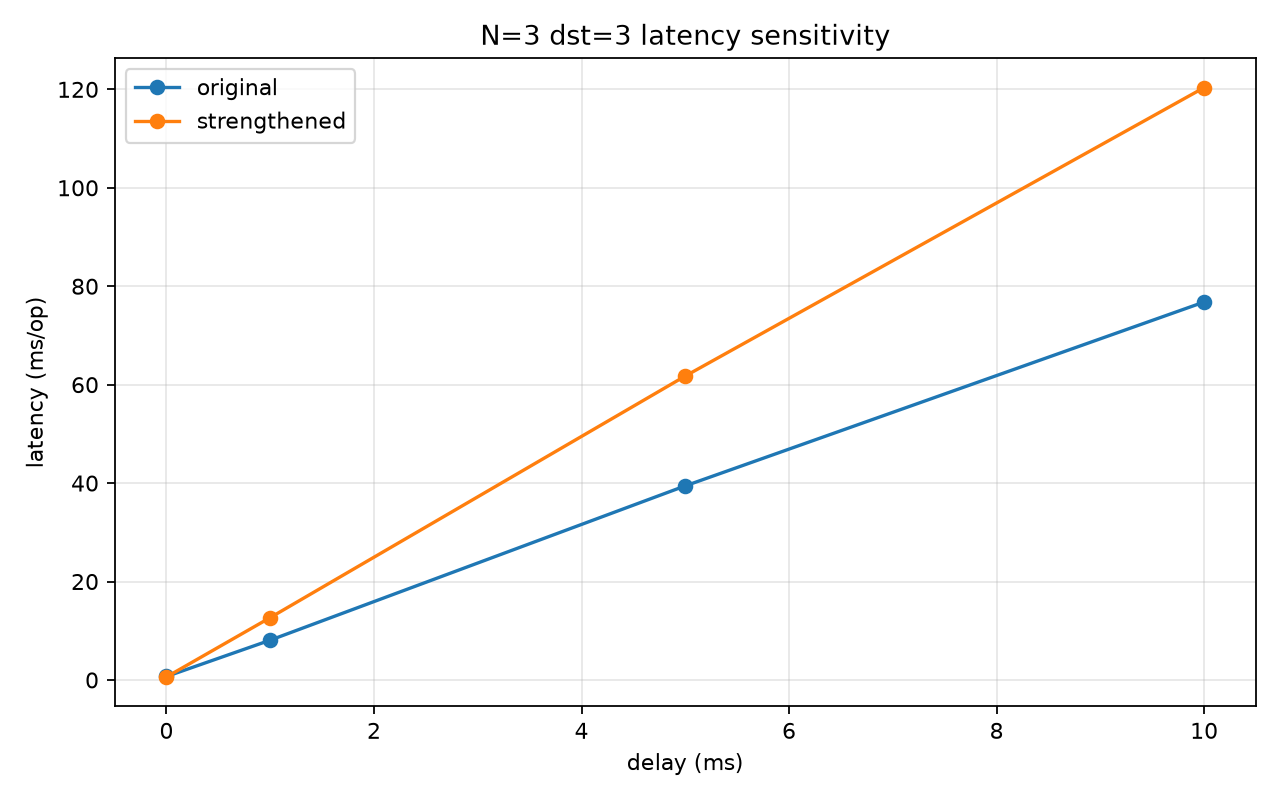
\includegraphics[width=\linewidth,keepaspectratio]{latency_vs_delay.png}
\caption{Per-operation latency for $N=3$, dst=3 under artificial protocol-message delay.}
\label{fig:latency}
\end{figure}

The zero-delay row in the latency benchmark is noisier than the dedicated in-memory benchmark because it is collected through the latency benchmark harness; therefore, Table~\ref{tab:inmemory} is the better baseline for CPU-only protocol overhead. The delayed rows are nevertheless useful because the same harness applies the same delay policy to both modes.

\subsection{ACK-Specific Delay}

Figure~\ref{fig:ackdelay} isolates ACK latency for the ACK-gated protocol. With no regular-message delay and only ACK messages delayed, the average operation time rises from $0.610 \pm 0.005$ ms at 0 ms ACK delay to $5.673 \pm 0.064$ ms at 1 ms, $29.648 \pm 1.045$ ms at 5 ms, and $58.860 \pm 2.389$ ms at 10 ms. In this implementation with destination count 3, an ACK-gated request may issue six peer ACK sends, since each of the three destinations sends ACKs to the other two destinations. A least-squares fit over the four ACK-delay means gives
\[
\mathrm{latency} \approx 0.256 + 5.860 \cdot \mathrm{ackDelay}
\]
with $R^2=0.9998$, close to the expected six-delay slope. This plot is therefore also a mechanism check: the measured latency increase is explained by the ACK sends placed on the critical path of the in-memory benchmark harness.

\begin{figure}[t]
\centering
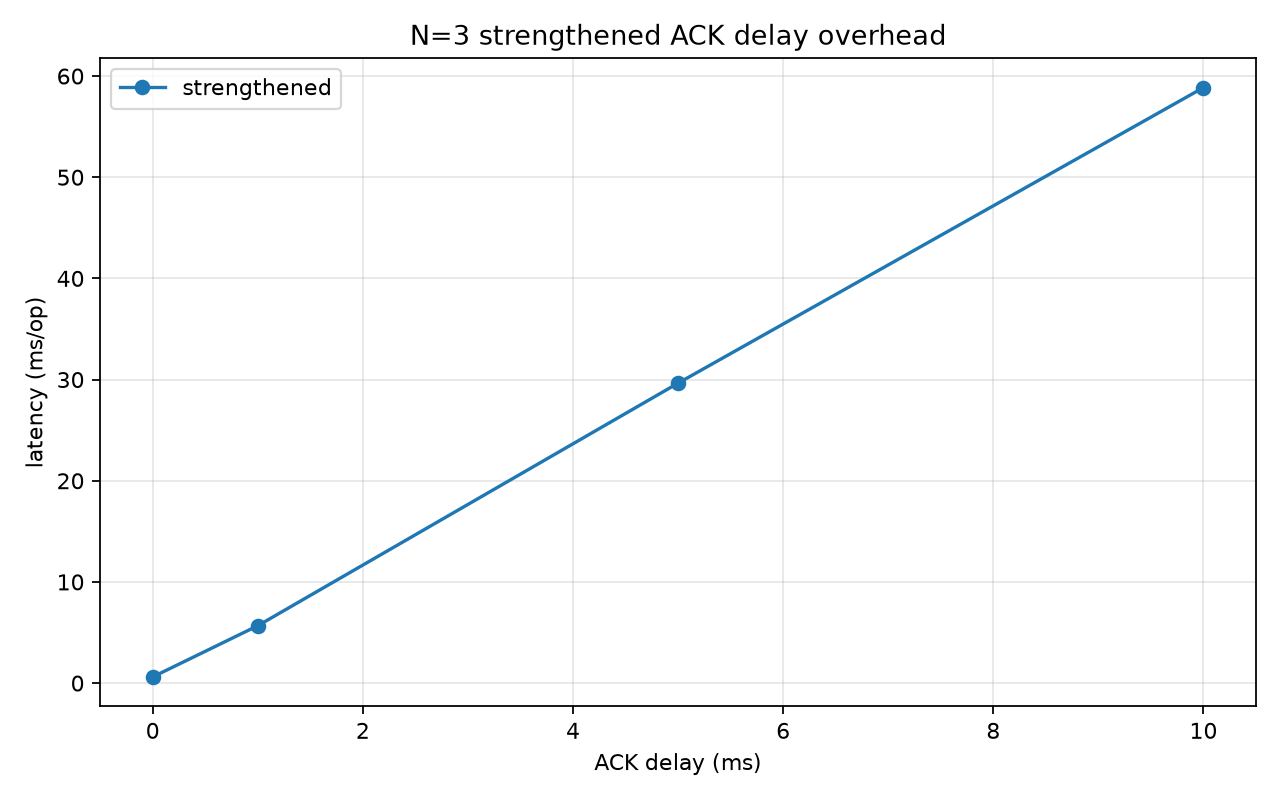
\includegraphics[width=\linewidth,keepaspectratio]{ack_delay_overhead.png}
\caption{Per-operation latency for $N=3$, dst=3 when artificial delay is applied only to ACK messages.}
\label{fig:ackdelay}
\end{figure}

\section{Discussion, Limitations, and Conclusion}

The results show a clear safety-performance trade-off across the three research questions. RQ1 is answered by the deterministic reproduction of the unsafe original-Skeen execution. RQ2 is answered by the identical schedule in ACK-gated mode, where the missing acknowledgement prevents the premature delivery that creates the cycle. RQ3 is answered by the overhead measurements: original Skeen is smaller and faster because delivery depends on timestamp stability alone, while ACK gating adds explicit coordination at the multicast layer. In low-latency in-memory settings, this cost is measurable but moderate. Under injected phase-counting latency, the additional ACK phase becomes the dominant difference.

This design is attractive when the application requires the stronger ordering property described by Pacheco et al. \cite{pacheco}. Without the ACK gate, the storage layer would need to compensate by coordinating during execution, which moves complexity out of the multicast layer and into every replicated operation path. ACK gating centralizes that responsibility in one delivery predicate.

The evaluation has several limitations. The prototype models one process per partition and assumes static membership. It does not implement replicated partition groups, crash recovery, persistent logs, view changes, or dynamic reconfiguration. The deterministic scheduler validates carefully selected traces rather than exhaustively exploring all schedules. The performance study is limited to $N \leq 5$ and artificial delay injection; larger clusters, real network jitter, packet loss, and failure recovery would need separate experiments.

\subsection{ACK-Gate Liveness}

The ACK gate strengthens safety by delaying delivery until every destination has acknowledged the final timestamp, but this also places ACK receipt on the liveness path. In the current implementation, which assumes no fail-stop failures, an ACK that is lost, delayed indefinitely, or never sent because a destination crashes can stall delivery forever for that request. There is no timeout-based suspicion, view change, retransmission protocol, persistent recovery, or quorum substitute for the all-destination ACK predicate. This limitation is a direct consequence of evaluating the protocol in a static, reliable-membership setting. A production design would need to combine the ACK gate with failure detection, membership reconfiguration, and recovery rules that preserve the ACK-gated ordering guarantee while preventing permanent starvation.

In conclusion, the project demonstrates that deterministic scheduling is a practical way to reproduce subtle distributed coordination bugs. By controlling message release with predicates and checking delivery graphs for cycles, the framework reproduces an unsafe original-Skeen execution without relying on sleeps or probabilistic races. The ACK-gated variant prevents that scheduled execution by requiring all destinations to acknowledge final timestamps before delivery. Benchmarks show that this safety improvement carries measurable overhead in local execution and substantial latency sensitivity when ACK messages are delayed, making the trade-off explicit for designers of partitioned state machine replication systems.

\documentclass[conference]{IEEEtran}

\usepackage[T1]{fontenc}
\usepackage[utf8]{inputenc}
\usepackage{amsmath}
\usepackage{amssymb}
\usepackage{graphicx}
\usepackage{booktabs}
\usepackage{cite}
\usepackage{url}
\usepackage{hyperref}

\graphicspath{{figures/}}

% arXiv source bundle note:
% Upload paper.tex and the files under figures/. The bibliography is embedded
% below with thebibliography, so BibTeX and external .bst files are not required.

\title{Robust Atomic Multicast: Evaluating ACK-Gated Skeen via Deterministic Protocol Validation}
\author{Agatha Schneider\\
Pontifícia Universidade Católica do Rio Grande do Sul (PUCRS)\\
Porto Alegre, Brazil\\
htaschneider@icloud.com
}
\date{}

\begin{document}

\maketitle

\begin{abstract}
Atomic multicast is a central communication abstraction for partitioned state machine replication and distributed key-value stores because it orders operations only at the partitions they access while preserving consistency across overlapping destination sets. Skeen's decentralized atomic multicast protocol provides a compact timestamp-based ordering mechanism, but later work shows that the original protocol admits unsafe executions when overlapping multicasts expose real-time dependencies before all destinations have converged on the same delivery barrier. This paper presents an implementation and evaluation of two protocols in a distributed key-value store: the original Skeen protocol and the ACK-gated extension proposed by Pacheco et al. The system supports generic N-partition routing, configurable membership, arbitrary multicast destination sets, in-memory and HTTP transports, Docker deployment, and structured logging. Our main engineering contribution is a deterministic validation framework that controls message delivery using scheduled transport queues, predicate-based release rules, delivery trace recording, and cycle detection. The framework reproduces the unsafe execution for original Skeen without sleeps or timing races and shows that the ACK-gated variant prevents premature delivery under the same schedule. We also benchmark both protocols for cluster sizes 2, 3, and 5 and destination sets up to the full cluster under injected delays of 0, 1, 5, and 10 ms. The results quantify the cost of the acknowledgement barrier: the strengthened protocol adds modest CPU and allocation overhead in the zero-delay case, but the extra control-message dependency becomes visible under artificial latency.
\end{abstract}

\section{Introduction}

Distributed key-value stores and partitioned state machine replication systems must often coordinate operations that access only a subset of partitions. A single-key update may involve one partition, whereas a range query or multi-key transaction may span several partitions. Broadcasting every operation to every server is simple but wasteful; routing each operation only to its destination set improves scalability but requires a multicast layer that preserves a consistent order whenever destination sets overlap.

Atomic multicast addresses this requirement by ensuring that processes delivering the same messages deliver them in the same order. Skeen's protocol is a classic decentralized solution based on logical timestamps, local timestamp proposals, a final timestamp decision, and delivery queues ordered by final sequence numbers \cite{skeen}. Its appeal is that it avoids a single sequencer and lets each multicast destination participate in timestamp selection.

However, Pacheco et al. show that global total order alone is not sufficient for partitioned state machine replication when real-time dependencies cross overlapping groups \cite{pacheco}. In particular, the original protocol can deliver a message at one destination, accept a later overlapping multicast, and then allow another destination to observe the later message before the earlier one. The resulting execution may be compatible with each local delivery queue but incompatible with the stronger atomic global order needed to avoid application-level coordination.

This paper evaluates that issue through an independent implementation rather than only a proof sketch. We implement both original Skeen and the ACK-gated strengthened variant in a distributed key-value store, validate the known unsafe execution using a deterministic scheduler, and measure the cost of adding the acknowledgement barrier.

The contributions are:
\begin{itemize}
    \item A configurable distributed key-value store with generic partition routing, static membership configuration, arbitrary multicast destination sets, and selectable original or strengthened Skeen modes.
    \item A dual transport stack with an in-memory transport for tests and controlled simulation, an HTTP transport for deployment, Docker configuration, and logging abstractions.
    \item A deterministic validation framework that reproduces the unsafe original-Skeen execution using scheduled message delivery, predicate-based release, delivery recording, and cycle detection.
    \item A benchmark pipeline that collects Go benchmark output, parses it into CSV matrices, and generates Matplotlib plots for throughput, memory consumption, allocation rate, and latency sensitivity.
\end{itemize}

The evaluation is organized around three research questions. \textbf{RQ1}: Can the unsafe execution described for original Skeen be reproduced in an independent implementation? \textbf{RQ2}: Does the ACK-gated extension eliminate the same execution under an identical deterministic schedule? \textbf{RQ3}: What CPU, memory, allocation, and latency overheads does the acknowledgement barrier introduce?

\section{Background and Related Work}

Atomic multicast provides reliable, consistently ordered delivery to a subset of processes. If two multicast messages are delivered at two common destinations, those destinations must deliver them in the same relative order. This property is especially useful in partitioned storage systems: each operation is multicast only to the partitions whose state it may read or write, but overlapping operations still observe a common serialization order.

Skeen's protocol assigns total order without a centralized sequencer \cite{skeen}. A client or coordinator sends a \textsc{Start} message to every destination in the multicast set. Each destination increments a logical clock, stores the request in a delivery queue as undeliverable, and returns a proposed timestamp. After proposals have been collected, the maximum proposed timestamp becomes the final timestamp. The final timestamp is multicast to all destinations, and a process may deliver the message when it is stable at the head of its queue. Ties are broken by process identifiers, producing a deterministic ordering relation over timestamp pairs.

The vulnerability identified by Pacheco et al. is not simply a disagreement about the final timestamp of one message \cite{pacheco}. The problem appears when real-time dependencies interact with overlapping destination sets. Suppose message $m$ is delivered at one destination before a later message $m'$ is multicast, but another destination learns enough timestamps to deliver $m'$ before $m$. The local delivery rules can remain internally consistent while the global execution graph contains a cycle: a real-time edge $m \rightarrow m'$ and a delivery-order edge $m' \rightarrow m$. This violates the stronger ordering needed by partitioned state machine replication to execute delivered operations immediately without additional synchronization.

The ACK-gated extension strengthens delivery by adding an explicit acknowledgement barrier after the final timestamp is learned. Once a destination learns the final timestamp, it broadcasts an \textsc{ACK} to the other destinations. A message is deliverable only after the process has received acknowledgements from every destination in the multicast set. This barrier prevents a destination from delivering a finalized message while another destination in the same multicast is still able to assign or expose a lower ordering constraint for an overlapping execution.

\section{System Architecture and Implementation}

\subsection{Distributed Key-Value Store}

The implementation exposes a partitioned key-value store over the multicast abstraction. Requests carry an operation type, request identifier, and explicit destination set. \textsc{Put} operations target exactly one partition, while range operations may target arbitrary destination sets. The routing layer supports configurable $N$-partition clusters, so the same protocol code can be evaluated for $N=2$, $N=3$, and $N=5$ without hard-coded participant assumptions.

% arXiv figure placeholder: insert the system architecture diagram here when available.
% Store the asset as figures/architecture.pdf for vector output or figures/architecture.png for raster output.
% Use a relative path only, for example:
% \begin{figure}[t]
% \centering
% \includegraphics[width=\linewidth,keepaspectratio]{figures/architecture.pdf}
% \caption{Distributed key-value store architecture and transport abstraction.}
% \label{fig:architecture}
% \end{figure}
% If using PNG, export with a tight bounding box and enough whitespace inside the image so labels are not clipped.

Each partition owns a Skeen protocol instance, a local key-value store, a logical clock, and a map of request states. A request state records the request payload, the local timestamp proposal, all collected proposals, the final timestamp, ACK state, delivery status, result data, and a completion channel used by synchronous client submission. Protocol mode is selected at construction time: original mode ignores ACK state during delivery, while strengthened mode requires every destination ACK before delivery.

\subsection{Protocol Execution}

The implementation uses four protocol message types: \textsc{Start}, \textsc{Local\_TS}, \textsc{Final\_TS}, and \textsc{ACK}. On \textsc{Start}, a destination validates membership in the destination set, advances its clock, stores a local proposal, and broadcasts that proposal. When proposals from all destinations are present, the maximum timestamp is learned as the final timestamp and broadcast. A final timestamp also advances local clock state if necessary.

% arXiv figure placeholder: insert the protocol timeline diagram here when available.
% Store the asset as figures/protocol-timeline.pdf for vector output or figures/protocol-timeline.png for raster output.
% Use a relative path only, for example:
% \begin{figure}[t]
% \centering
% \includegraphics[width=\linewidth,keepaspectratio]{figures/protocol-timeline.pdf}
% \caption{Timeline of original Skeen and ACK-gated message phases.}
% \label{fig:protocol-timeline}
% \end{figure}
% Prefer PDF/SVG-converted-to-PDF for sequence diagrams; if using PNG, crop to the diagram boundary and avoid external bounding-box options.

Delivery is attempted after every protocol message. The node collects finalized, undelivered requests and sorts them by final timestamp. A candidate can be delivered only if it is finalized, not already delivered, and lower than every other pending local or final timestamp known at the node. In strengthened mode, the same candidate must also have ACKs from all destinations. Delivery executes the key-value operation, records any range result, invokes the delivery hook used by tests, and releases the waiting submitter.

\subsection{Dual Transport Stack and Deployment}

The transport interface contains a single protocol send operation. The in-memory transport maps partition identifiers directly to local Skeen instances and is used for unit tests, benchmarks, and deterministic simulation. The HTTP transport serializes protocol messages as JSON and sends them to each peer partition's internal protocol endpoint. This separation lets the protocol be tested without network non-determinism while preserving a deployable HTTP path. The repository also includes Docker Compose configurations for multi-process execution and logging helpers that can be disabled during benchmarks.

\subsection{Deterministic Validation Framework}

Distributed protocol tests frequently rely on sleeps, goroutine scheduling, or best-effort network delays. Those techniques make unsafe traces difficult to reproduce and can confuse protocol bugs with timing accidents. Our validation framework instead introduces a scheduled transport that records outbound protocol messages rather than delivering them immediately. Tests explicitly release queued messages through predicates over message type, request identifier, sender, receiver, and destination set.

The framework also records per-partition delivery traces. These traces are converted into a directed graph: if a partition delivers $a$ before $b$, the graph records $a \rightarrow b$. Tests may add real-time edges from the scenario under study, such as $m \rightarrow m'$ when $m'$ is submitted only after $m$ has already been delivered. A depth-first cycle detector then determines whether the combined delivery and real-time constraints violate atomic global order.

The reproduced unsafe schedule uses three partitions. Message $m$ targets partitions 0 and 1; message $m'$ targets partitions 0 and 2. By controlling initial clocks and releasing selected \textsc{Local\_TS} messages, the original protocol allows partition 1 to deliver $m$, then allows partition 0 to deliver $m'$ before $m$. Adding the real-time edge from the delivery of $m$ to the later multicast of $m'$ creates the expected cycle. Running the same schedule in strengthened mode leaves partition 1 unable to deliver $m$ until the missing destination ACK is released; after the scheduler drains all messages, no cycle is detected.

\section{Experimental Evaluation}

\subsection{Methodology}

The benchmark pipeline begins with Go benchmarks using \texttt{testing.B} and \texttt{ReportAllocs}. Raw benchmark text is converted to CSV by a custom parser that extracts benchmark name, cluster size, protocol mode, destination count, fixed delay, ACK-specific delay, \texttt{ns/op}, \texttt{B/op}, and \texttt{allocs/op}. The plotting stage loads these matrices and generates high-resolution PNG plots with Matplotlib.

Two benchmark families are used. The first evaluates destination-set overhead for $N \in \{2,3,5\}$ and destination counts from one partition to the full cluster. The second fixes $N=3$ and injects artificial latency of 0, 1, 5, and 10 ms into protocol messages. A separate ACK-delay benchmark applies delay only to \textsc{ACK} messages, isolating the cost of the strengthened protocol's additional barrier.

\subsection{Correctness Results}

The deterministic validation tests answer RQ1 and RQ2. Original Skeen reproduces the unsafe Pacheco-style trace: one partition delivers $m$, a later overlapping multicast $m'$ is introduced, and another partition delivers $m'$ before $m$. The resulting graph contains a cycle once the real-time edge $m \rightarrow m'$ is included. A control test also verifies that original Skeen does not create a pure delivery-order cycle without the real-time edge, matching the nature of the reported vulnerability.

The ACK-gated implementation prevents the same trace. Under the identical message schedule, a destination that has learned a final timestamp cannot deliver until every destination in the multicast set has acknowledged that final timestamp. This blocks the premature delivery that creates the original cycle. Once the scheduler drains all messages, delivery proceeds consistently and the cycle detector reports no violation.

\subsection{Zero-Delay Overhead}

Table~\ref{tab:inmemory} summarizes the in-memory destination-overhead benchmark. With full destination sets, strengthened mode increases latency from 0.293 ms to 0.350 ms at $N=2$, from 0.488 ms to 0.608 ms at $N=3$, and from 0.751 ms to 1.193 ms at $N=5$. The cost is also visible in memory and allocation counters because ACK state and ACK messages add per-request bookkeeping.

\begin{table}[t]
\centering
\caption{In-memory full-destination overhead. Values are means over the parsed benchmark runs.}
\label{tab:inmemory}
\begin{tabular}{lrrrr}
\toprule
Mode / $N$ & dst & ms/op & B/op & allocs/op \\
\midrule
Original / 2 & 2 & 0.293 & 5039 & 53.1 \\
Strengthened / 2 & 2 & 0.350 & 7214 & 71.0 \\
Original / 3 & 3 & 0.488 & 8074 & 72.0 \\
Strengthened / 3 & 3 & 0.608 & 12292 & 104.1 \\
Original / 5 & 5 & 0.751 & 16208 & 110.0 \\
Strengthened / 5 & 5 & 1.193 & 26320 & 176.0 \\
\bottomrule
\end{tabular}
\end{table}

\begin{figure}[t]
\centering

\includegraphics[width=\linewidth,keepaspectratio]{figures/overhead_by_dst.png}
\caption{Destination-set overhead for $N=3$ without artificial latency.}
\label{fig:overhead}
\end{figure}

Figure~\ref{fig:overhead} shows that the ACK gate has almost no effect for single-destination operations, where the process can acknowledge itself, but the gap grows with destination-set size. This matches the implementation structure: the strengthened protocol only adds meaningful network fan-out when more than one destination participates.

\subsection{Latency Sensitivity}

Table~\ref{tab:latency} and Fig.~\ref{fig:latency} evaluate $N=3$, destination count 3, and fixed artificial delay on all protocol messages. At 5 ms injected delay, original Skeen averages 39.436 ms/op while strengthened Skeen averages 61.753 ms/op. At 10 ms, the original protocol averages 76.789 ms/op and the strengthened protocol averages 120.357 ms/op. The additional delay is consistent with the extra ACK dependency: the strengthened protocol is not only performing more local bookkeeping, it must also wait for another control-message phase before delivery can release the client operation.

\begin{table}[t]
\centering
\caption{$N=3$, dst=3 latency sensitivity under fixed artificial message delay.}
\label{tab:latency}
\begin{tabular}{lrrrr}
\toprule
Mode & delay (ms) & ms/op & B/op & allocs/op \\
\midrule
Original & 0 & 0.706 & 8076 & 71.8 \\
Strengthened & 0 & 0.615 & 12302 & 104.2 \\
Original & 1 & 8.085 & 12582 & 126.0 \\
Strengthened & 1 & 12.670 & 18357 & 176.0 \\
Original & 5 & 39.436 & 12733 & 127.0 \\
Strengthened & 5 & 61.753 & 18496 & 177.8 \\
Original & 10 & 76.789 & 12773 & 128.0 \\
Strengthened & 10 & 120.357 & 18594 & 178.8 \\
\bottomrule
\end{tabular}
\end{table}

\begin{figure}[t]
\centering

\includegraphics[width=\linewidth,keepaspectratio]{figures/latency_vs_delay.png}
\caption{$N=3$, dst=3 sensitivity to artificial protocol-message delay.}
\label{fig:latency}
\end{figure}

The zero-delay row in the latency benchmark is noisier than the dedicated in-memory benchmark because it is collected through the latency benchmark harness; therefore, Table~\ref{tab:inmemory} is the better baseline for CPU-only protocol overhead. The delayed rows are nevertheless useful because the same harness applies the same delay policy to both modes.

\subsection{ACK-Specific Delay}

Figure~\ref{fig:ackdelay} isolates ACK latency for the strengthened protocol. With no regular-message delay and only ACK messages delayed, the average operation time rises from 0.610 ms at 0 ms ACK delay to 5.673 ms at 1 ms, 29.648 ms at 5 ms, and 58.860 ms at 10 ms. This result confirms that the acknowledgement barrier is on the critical path for multi-destination requests.

\begin{figure}[t]
\centering

\includegraphics[width=\linewidth,keepaspectratio]{figures/ack_delay_overhead.png}
\caption{$N=3$, dst=3 overhead when artificial delay is applied only to ACK messages.}
\label{fig:ackdelay}
\end{figure}

\section{Discussion, Limitations, and Conclusion}

The results show a clear safety-performance trade-off. Original Skeen is smaller and faster because delivery depends on timestamp stability alone. The strengthened protocol adds explicit coordination at the multicast layer, which prevents the reproduced unsafe execution and lets the key-value layer execute delivered operations without adding its own cross-partition barrier. In low-latency in-memory settings, this cost is measurable but moderate. Under injected latency, the additional ACK phase becomes the dominant difference.

This design is attractive when the application requires the stronger ordering property described by Pacheco et al. \cite{pacheco}. Without the ACK gate, the storage layer would need to compensate by coordinating during execution, which moves complexity out of the multicast layer and into every replicated operation path. The strengthened protocol centralizes that responsibility in one delivery predicate.

The evaluation has several limitations. The implementation models one process per partition and assumes static membership. It does not implement replicated partition groups, crash recovery, persistent logs, view changes, or dynamic reconfiguration. The deterministic scheduler validates carefully selected traces rather than exhaustively exploring all schedules. The performance study is limited to $N \leq 5$ and artificial delay injection; larger clusters, real network jitter, packet loss, and failure recovery would need separate experiments.

In conclusion, the project demonstrates that deterministic scheduling is a practical way to validate subtle distributed coordination bugs. By controlling message release with predicates and checking delivery graphs for cycles, the framework reproduces an unsafe original-Skeen execution without relying on sleeps or probabilistic races. The ACK-gated variant prevents that execution by requiring all destinations to acknowledge final timestamps before delivery. Benchmarks show that this safety improvement carries moderate overhead in local execution and substantial latency sensitivity when ACK messages are delayed, making the trade-off explicit for designers of partitioned state machine replication systems.

\begin{thebibliography}{1}

\bibitem{skeen}
D.~Skeen, ``A decentralized formalism for agreement protocols,'' in
\emph{Proceedings of the IEEE Symposium on Reliability in Distributed Software
and Database Systems}, 1981, pp. 123--134.

\bibitem{pacheco}
N.~Pacheco \emph{et al.}, ``Correcting and enhancing decentralized atomic
multicast algorithms,'' \emph{IEEE Transactions on Parallel and Distributed
Systems}, vol.~34, no.~5, pp. 1420--1432, 2023.

\end{thebibliography}

\end{document}


\end{document}
\typeout{get arXiv to do 4 passes: Label(s) may have changed. Rerun}
